\documentclass{article}\usepackage{multirow}\usepackage{changepage}\usepackage{graphicx}\usepackage{amsmath}\usepackage{amssymb}\title{Young's Double Slit}\author{Tristan Simpson}\begin{document}\maketitle\section{Notes}\begin{itemize}\item {the longer the wave lengths, the farther the interference pattern is.}\item {the shorter the wave length, the shorter the interference pattern is.}\item {florescant lights: put fingers close together act like a slit}\item {thrusday is young's double slit experiment}\item {monochromatic light you see either light or dark}\item {light from sun you see white in center then colors on the side depending on how the waves decontrustive and construvely interfere}\item {by rotating the wave in a slit, the wave distances between the two waves (original wave and reflected wave) changes}\item {minima is when a crest and a trough align with eachother, cancelling eachother out}\item {maxima is when a crest and crest or trough and trough align with eachother}\item {angle from dark region formula: $\sin \theta_{n} = (n - \frac{1}{2})\frac{\lambda}{d}; n = 1, 2, 3...$}\item {angle from bright region formula: $\sin \theta_{m} = \frac{m\lambda}{d}; m = 1, 2, 3...$}\item {distance between adjacent nodal lines: $\Delta x$ as $\frac{\Delta x}{L} = \frac{\lambda}{d}$}\item {young's double slit you have a central maxima then all the rest are evenely spaced on the other side.}\item {single slit: double width in center, single width on the sides}\item {diffraction grading: all same intensity, small minimas and large maximas. All evenly spread out.}\item {Must explain why the above happens for test.}\end{itemize}\leavevmode\section{Homework}\begin{adjustwidth}{0cm}{0pt}{Two slits produce an interference pattern. The distance between the slits and the screen is 7.7m. The two third-order maxima are separated from each other by a distance of $32.9 \times 10^{-2} m$. The wavelength of the light is $4.9 \times 10^{-7} m$. Calculate the separation between the slits.}\end{adjustwidth}\leavevmode\\\begin{equation}\Delta\;x\;=\;(L)\left(\frac{\lambda}{d}\right)\end{equation}\begin{equation}\Delta\;x\;=\;(32.9\;\times\;10^{-2})\left(\frac{4.9\;\times\;10^{-7}}{7.7}\right)\end{equation}\newline\begin{equation}\therefore\;\Delta\;x\;\approx\;2.01\;\times\;10^{-8}\end{equation}\newline\section{Images}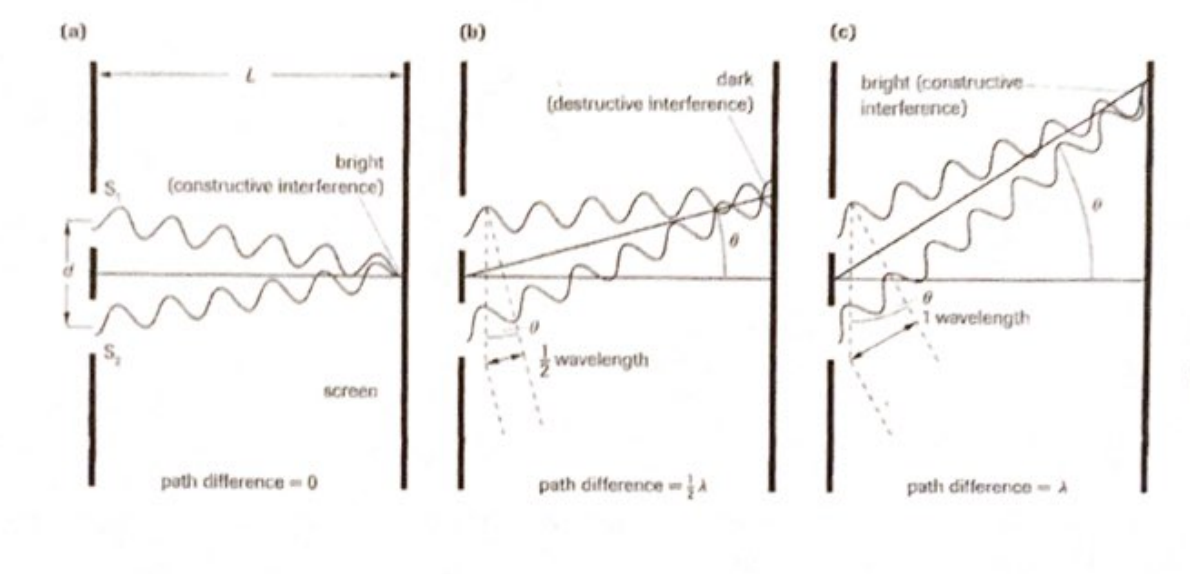
\includegraphics[scale=0.4]{/Users/tristan/Desktop/LaTeX/Hidden/ratex//images/light.png}\end{document}